%% Introduction: problem, missing evaluation dimension, phenomenon, insight, method, supporting mechanisms,
%% results, and three contributions. See CLAUDE_paper.md section 6.
%% Included by sigconf.tex. Do not add a preamble here.

\section{Introduction}
Irregular sampling is a property of how temporal systems are recorded, not of the systems themselves. A
laboratory value exists in a patient's record because a clinician ordered it; a weather station reports at the
rate its hardware and maintenance schedule permit; a wearable device logs motion only while it has contact and
power. In each case the data are the outcome of two processes: the temporal dynamics of the system, and the
\emph{observation process} that samples them.

A large literature builds encoders for the resulting data, including recurrent models with decay
\cite{che2018grud}, continuous-time latent models \cite{rubanova2019latentode,debrouwer2019gruodebayes,kidger2020ncde},
set-function and attention aggregation \cite{horn2020seft,shukla2021mtand}, graph-guided models
\cite{zhang2022raindrop,zhang2024tpatchgnn} and query-based embeddings that let standard multivariate backbones
consume irregular observations directly \cite{lim2026quite}. These methods differ in how they represent a
\emph{given} set of observations, and each is trained and evaluated under one observation process: the one the
benchmark happens to encode. The observation process, however, is not fixed by the domain. Another hospital
orders panels on another schedule, a sensor network is redeployed with a new sampling policy, a firmware update
changes when readings are written. We call this \emph{observation-process shift}: $P(\Sobs)$ moves while the
underlying dynamics $P(X)$ stay comparable, and a protocol that draws train and test data from a single
observation process cannot see it.

\begin{figure}[t]
\centering
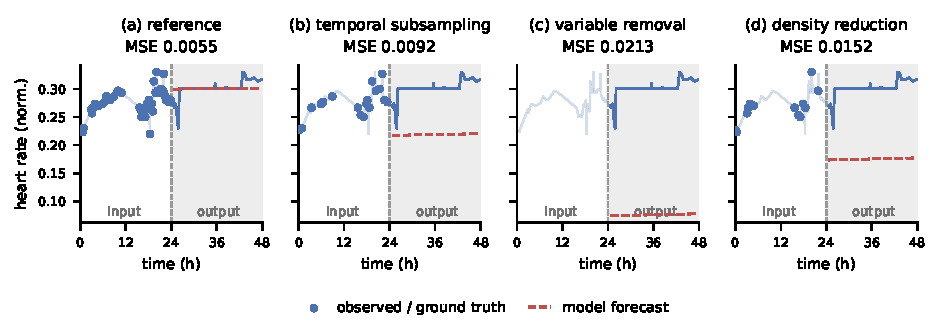
\includegraphics[width=\linewidth]{figures/fig2_observation_shift.pdf}
\caption{The same ICU history (heart rate and mean arterial pressure over 24\,h) observed through four
observation processes. The faint trajectory shows the underlying observations; markers indicate what the model
receives. The underlying history and the prediction target are identical across panels --- only the observation
process changes, moving one dimension of it at a time: how often measurements arrive (b), which variables are
recorded (c), and how many survive (d). The forecasting MSE of the same model under each condition is annotated
in each panel\prelim, so the change in predictive performance is attributable to the observation process alone.
Panels (b)--(d) are the evaluation conditions of Section~\ref{sec:splits}.}
\label{fig:views}
\end{figure}

The shift is easy to measure and can be large. Re-observing only the \emph{history} of each held-out input
through a different admissible process, with the prediction targets untouched (Figure~\ref{fig:views}), raises
the error of a wearable-sensor forecaster by a factor of nineteen and of a clinical forecaster by a factor of
two, while leaving a climate forecaster essentially unaffected. Two controlled comparisons sharpen this.
Observation density does not determine the damage: among processes that each delete about half of the
observations, error varies by up to $3.8\times$ depending on which half. And the damaging \emph{kind} of loss is
modality-dependent, with removal of whole variables dominating on clinical records and temporal subsampling
dominating on body-sensor records. A method that treats irregularity as a scalar corruption level cannot
represent either observation.

The starting point for our method is an asymmetry between training and deployment. At deployment the model is
given whatever the observation process supplies, and no more. During training, however, the same history can be
re-observed as often as we like, including through a process \emph{richer} than the one the model will face.
That richer observation is never available at test time, which makes it privileged information in the sense of
Learning Using Privileged Information \cite{vapnik2015lupi}: a training-time signal about the trajectory that the deployment view only partly
reveals.

We turn this into a training mechanism we call \emph{privileged observation self-distillation} (POSD). A teacher
$f_{\theta_T}$ receives a rich observation $\Sobs_{\mathrm{rich}}(X)$ of a history; a student $f_\theta$
receives a sparse observation $\Sobs(X)$ of the \emph{same} history, over the same prediction times and with the
same supervision; and the student is trained to match the teacher's task-level output in addition to the ground
truth. The teacher is not a larger or better-trained model, and it does not solve a different problem: it is the
same predictive model family with more information about the same trajectory. Its output therefore encodes what
is predictable from that trajectory when less of it has been discarded, which is exactly the target the student
should aim at from its restricted view. The teacher, the rich view and its extra forward pass all disappear
after training.

POSD is supported by a second mechanism and, conditionally, a third. \emph{Observation-process augmentation}
draws several observation processes per training trajectory from a mixture and trains on all of the resulting
views, treating the process as nuisance variation to randomise over; it is what exposes the student to process
variation in the first place, and it is the source of most of the robustness we measure. \emph{Hard
observation-process mining} instead searches a constrained candidate pool for the admissible process the current
model handles worst. Because its benefit turns on a property of the candidate pool rather than of the mechanism,
we keep it out of the headline configuration: 	extbf{OPERA} is augmentation plus privileged distillation, and
	extbf{OPERA++} adds mining from a pool strictly harsher than the training mixture.

Empirically, augmentation reduces relative degradation under shift from $+107\%$ to $+14\%$ on clinical
forecasting and from $+1793\%$ to $+25\%$ on wearable-sensor forecasting while leaving clean error unchanged, and
it transfers to observation-process \emph{families} that never appear in training. POSD adds a complementary
gain where augmentation alone does not help: on climate forecasting it improves clean error from $0.5329$ to
$0.5135$ and shifted error on every condition, and on sepsis prediction the complete configuration raises clean
AUROC from $82.1$ to $85.6$. Parameter count and inference latency are unchanged throughout.

\paragraph{Contributions.}
\begin{itemize}
\item \textbf{Observation-process shift.} We formalise observation-process shift as a distinct source of
distribution shift for irregular time series, give a composable removal-only family of observation processes
with validity constraints, and define a controlled protocol that re-observes held-out histories while preserving
targets, together with a train/test split over process families that makes generalisation measurable
(Sections~\ref{sec:problem} and \ref{sec:setup}).
\item \textbf{Privileged observation self-distillation.} We introduce a training mechanism in which a richer
observation of the same history supplies privileged task-level supervision to a student restricted to the
deployment observation, and we state and verify the invariant that separates it from label leakage: teacher and
student may differ only in the observation of the history (Section~\ref{sec:method}).
\item \textbf{Empirical robustness and its boundaries.} Across forecasting and classification benchmarks we show
that exposure to diverse observation processes substantially improves robustness, that privileged distillation
provides a complementary gain concentrated on information-limited tasks, and that hard mining helps only when its
candidate pool contains processes harsher than those augmentation already supplies (Section~\ref{sec:results}).
\end{itemize}

We use a query-based irregular encoder \cite{lim2026quite} as the experimental substrate because it consumes
irregular observations natively. Nothing in the formulation depends on that choice, and we report results on a
second backbone.
